\section{Annotation Schemas}
Users can upload their annotation schemas in XML format to the server so that 
they can be used in the process of manual annotation. Click on the 
$Resources >> Annotation Schemas$ option from the top menu and you will reach 
the annotation schema list page, as shown in Figure~\ref{fig:annoschemalist}.
\begin{figure}[ht!]
\centering
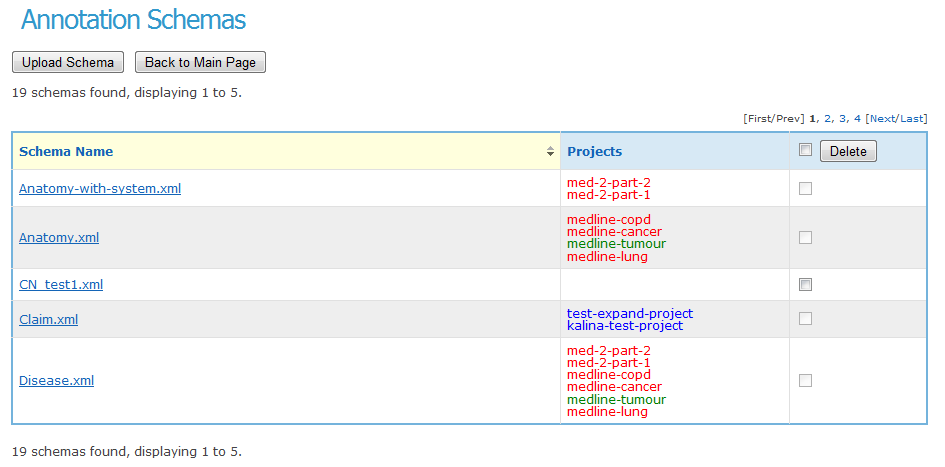
\includegraphics[scale=0.4]{annoschemalist}
\caption{Annotation Schema List}
\label{fig:annoschemalist}
\end{figure}

You can see if some annotation project, using particular schema is
running, suspended or finished. The links to the annotation
project statistics can be of different colours, depending on project status:
\emph{red}: suspended; \emph{blue}: running; \emph{green}: completed. More about
project statistics you can find in the next chapter.

To upload a new annotation schema to the server, click on the 
\emph{Upload Schema} button and you should reach the page where you can 
select the schema file on your file system (see Figure ~\ref{fig:addschema}).
\begin{figure}[ht!]
\centering
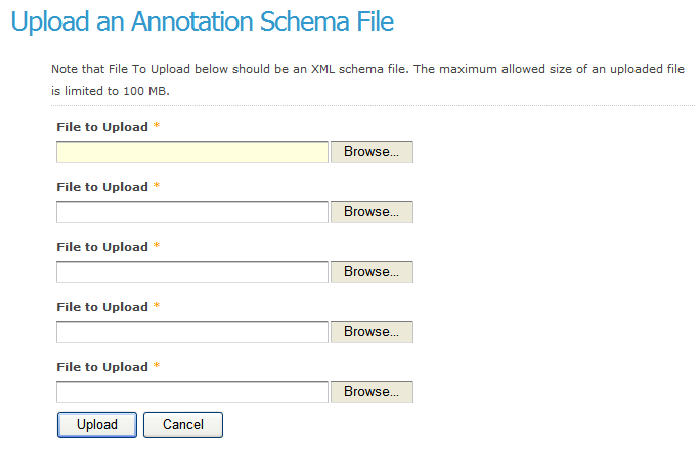
\includegraphics[scale=0.4]{addschema}
\caption{Upload Annotation Schema}
\label{fig:addschema}
\end{figure}

After clicking on the \emph{Save} button from , you will see
the confirmation message and the annotation schema you have added.

To delete one or more schemas, check the tickbox in the last column of the 
table (see Figure ~\ref{fig:annoschemalist})  and click \emph{Delete}. 

If you want to view annotation schema click on \emph{View} icon.

\section{Annotation Services}
Users with \emph{Administrator} role can view, add, update, and delete
annotation services. To view available annotation services, select
\emph{Services} option from \emph{Resources} menu
(see Figure~\ref{fig:annotationservices} below).
\begin{figure}[hb!]
\centering
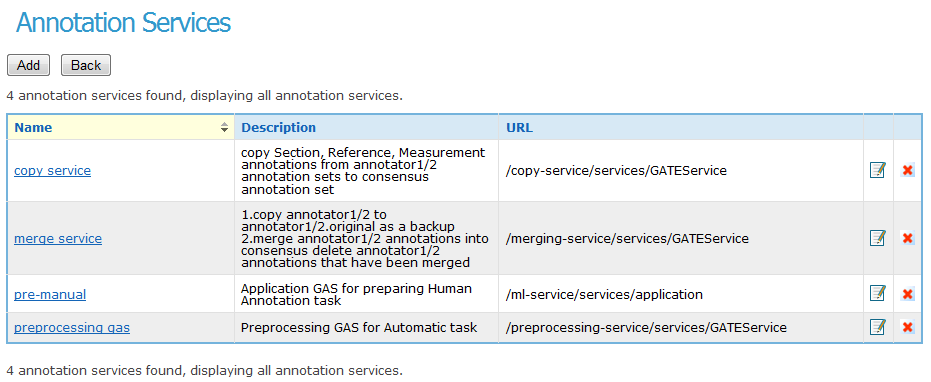
\includegraphics[scale=0.4]{annotationservices}
\caption{Annotation Services}
\label{fig:annotationservices}
\end{figure}

Here you can delete or update existing annotation services or create a new one.
Note that currently, GATE Teamware supports only GATE services (GAS).

To create a new GAS service, click on \emph{Add} button and fill in the form as
shown in Figure~\ref{fig:createannotationservice}.
\begin{figure}[hb!]
\centering
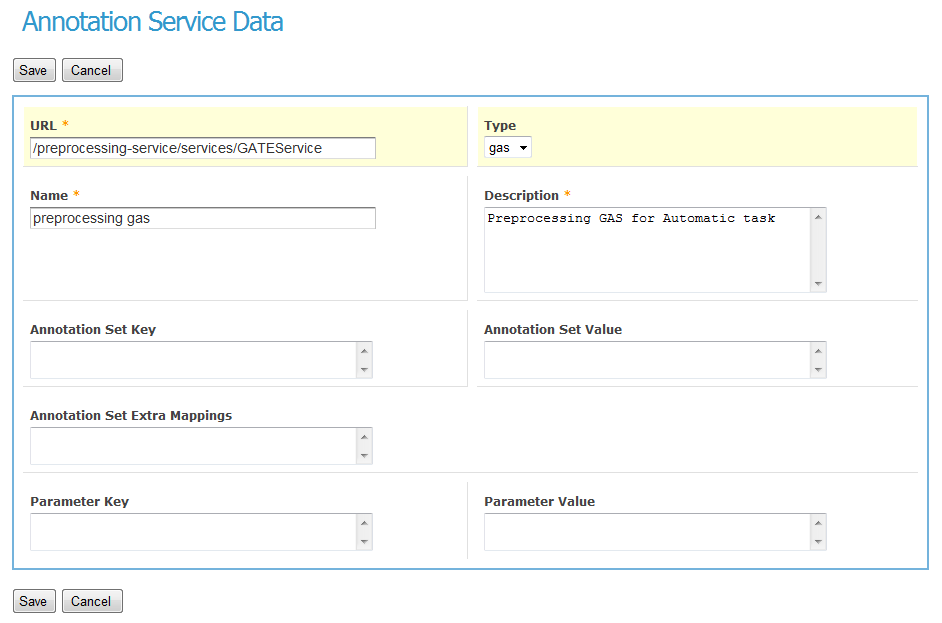
\includegraphics[scale=0.38]{createannotationservice}
\caption{New Annotation Service}
\label{fig:createannotationservice}
\end{figure}

This form is used to inform Teamware about a published service -- the service
must already be deployed at a URL accessible to the Teamware server.  The GATE
user guide\footnote{\url{http://gate.ac.uk/userguide/sec:howto:export}}
explains how to save a GATE application in a suitable package for publishing as
a Teamware service.
%
% When we have tools to automate the zip -> war step, this section will need to
% be expanded, it is deliberately vague at the moment...
%

Mandatory fields are:
\begin{itemize}
  \item \emph{url}: the URL of the GAS service you have published;
  \item \emph{name}: the friendly title, you will refer to, when you
configure your \emph{Workflow Template};
  \item \emph{description}: a few words about what GAS is doing.
\end{itemize}

It is important to mention that if you ommit \emph{http} in the
URL, it will be assumed that GAS is published under the same context as the web
application.
For example on Figure~\ref{fig:createannotationservice}, the preprocessing-gas
has URL
\emph{/preprocessing-service/services/GATEService}. That means if GATE Teamware
is hosted on
\emph{http://somehost/teamware} the GAS URL will be resolved as:
\emph{
http://somehost/teamware/preprocessing-service/services/GATEService}.


